\documentclass[a4paper,12pt,twoside]{article} % Format de page
\usepackage{pstricks-add} % Cr\’eer des figures
\usepackage{pstricks,pst-node,graphicx}
\newsavebox\IBox
\begin{document}
\thispagestyle{empty}
\sbox\IBox{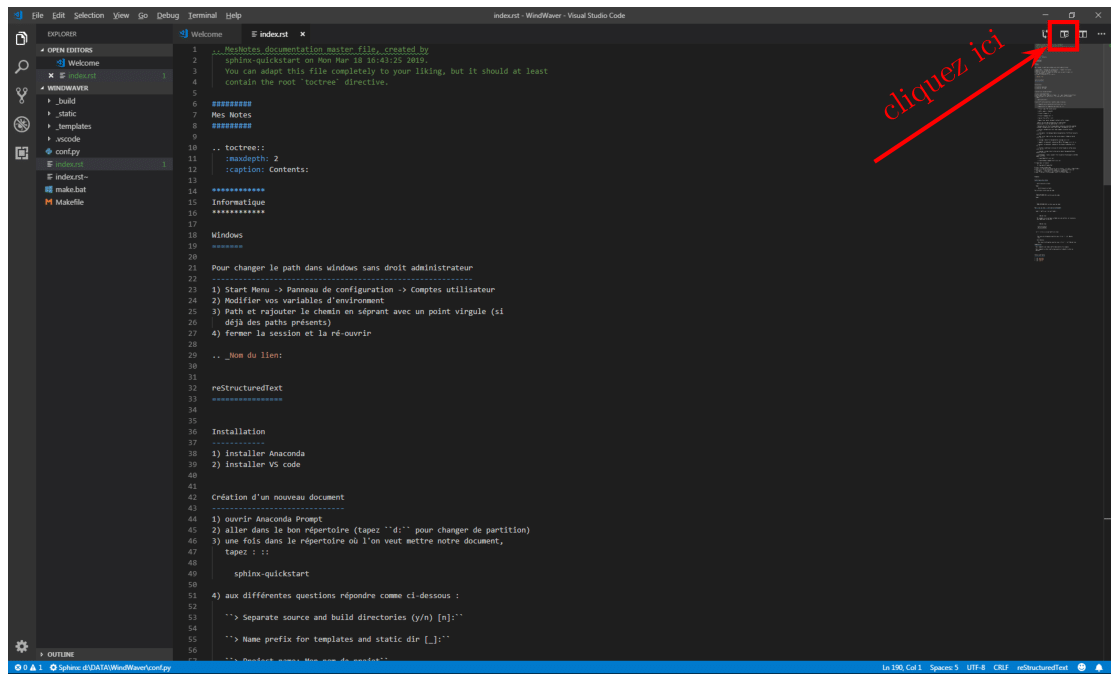
\includegraphics[width=14cm]{IconePrevisualisation.eps}}  
\begin{pspicture}(-0.5,-0.5)(\wd\IBox,\ht\IBox)
\rput[lb](0,0){\usebox\IBox}
%\psgrid[gridcolor=black!50,subgridcolor=black!15]
\psset{linecolor=red,linewidth=1.5pt,arrowscale=1.5,dotscale=1.5}
\fnode[framesize=0.4 0.4](13.4,8.1){A}
\pnode[11,6.5]{F}
% \rput(3.5,11.5){\ovalnode{F}{\textcolor{red}1}}
\ncline{->}{F}{A}
\aput{:U}{\textcolor{red}{cliquez ici}}
\end{pspicture}
\end{document}
